% !TeX root = main.tex

\section{Two-way Tables}

\hypertarget{two-way-frequency-tables}{%
\subsection{Two-way Frequency Tables}\label{two-way-frequency-tables}}

\begin{itemize}
\item
  As we organize and analyze data from two categorical variables, we
  make use of two-way tables.
\item
  Information in a \textbf{two-way frequency table}:

  \begin{itemize}
  \item
    Values of the two variables are displayed in the left column and the
    top row.
  \item
    The body of table consists of frequency counts associated to pairs
    of values of the two variables.
  \item
    The right column and the bottom row, which are called margins of the
    table, consists of row totals and column totals respectively.
  \end{itemize}
\item
  A number in a margin are called \textbf{marginal frequency}.
\item
  A numbers in the body of the table is called \textbf{joint frequency}.
\end{itemize}

\begin{example}

The following table summarize responses of a random sample of 1,200 U.S.
college students as part of a larger survey.

\begin{fullwidth}
  \colorbox{white}{
    \parbox{\linewidth}{\centering
  \begin{tabular*}{0.8\linewidth}{l*{4}{m{0.15\linewidth}}}
  \toprule
   & About Right
  & Overweight
  & Underweight
  & Row Totals\\
  \midrule
  Female & 560 & 163 & 37 & 760 \\
  Male & 295 & 72 & 73 & 440 \\
  Column Totals & 855 & 235 & 110 & 1,200 \\
  \bottomrule
  \end{tabular*}
  }}
\end{fullwidth}

\end{example}

\hypertarget{two-way-relative-frequency-tables-and-probability}{%
\subsection{Two-Way Relative Frequency Tables and
Probability}\label{two-way-relative-frequency-tables-and-probability}}

\begin{itemize}
\item
  A \textbf{two-way relative frequency table} is obtained from a two-way
  frequency table by converting frequencies in a two-way table to
  relative frequencies.
\item
  \textbf{Marginal probability}
  \[P(X)=\frac{\text{Marginal frequency in}~ X}{\text{Total}}\]
\item
  \textbf{Conditional probability}
  \[P(X|Y)=\frac{\text{Joint frequency}}{\text{Marginal Frequency in}~Y}\]
  \[P(Y|X)=\frac{\text{Joint frequency}}{\text{Marginal Frequency in}~X}\]
\item
  \textbf{Joint probability}
  \[P(X\text{and}~ Y)=\frac{\text{Joint frequency}}{\text{Total}}\]
\item
  Note that \(P(X~\text{and}~Y)=P(X)\cdot P(Y|X)=P(Y)\cdot P(X|Y).\)
\end{itemize}

\begin{example}

The following table shows joint and marginal probabilities of body image
and gender.

\begin{fullwidth}
  \colorbox{white}{
    \parbox{\linewidth}{\centering
  \begin{tabular*}{0.9\linewidth}{l*{4}{p{0.15\linewidth}}}
  \toprule
  & About Right
  & Overweight
  & Underweight
  & Row Totals\\
  \midrule
  Female & \(\frac{560}{1200}=46.67\%\) &
  \(\frac{163}{1200}=13.58\%\) & \(\frac{37}{1200}=3.08\%\) &
  \(\frac{760}{1200}=63.33\%\) \\
  Male & \(\frac{295}{1200}=24.58\%\) & \(\frac{72}{1200}=6.00\%\) &
  \(\frac{73}{1200}=6.08\%\) & \(\frac{440}{1200}=36.67\%\) \\
  Column Totals & \(\frac{855}{1200}=71.25\%\) &
  \(\frac{235}{1200}=19.58\%\) & \(\frac{110}{1200}=9.17\%\) &
  \(\frac{1200}{1200}=100.00\%\) \\
  \bottomrule
  \end{tabular*}
}}
\end{fullwidth}

\end{example}

\begin{example}

The following table shows probabilities of randomly select male or
female who has a certain body image.

\begin{fullwidth}
  \colorbox{white}{
    \parbox{\linewidth}{\centering
  \begin{tabular*}{0.8\linewidth}{l*{4}{m{0.15\linewidth}}}
  \toprule
  & About Right
  & Overweight
  & Underweight
  & Row Totals\\
  \midrule
  Female & \(\frac{560}{760}=73.68\%\) & \(\frac{163}{760}=21.45\%\)
  & \(\frac{37}{760}=4.87\%\) & \(\frac{760}{760}=100.00\%\) \\
  Male & \(\frac{295}{440}=67.05\%\) & \(\frac{72}{440}=16.36\%\) &
  \(\frac{73}{440}=16.59\%\) & \(\frac{440}{440}=100.00\%\) \\
  \bottomrule
  \end{tabular*}
}}
\end{fullwidth}

\end{example}

\begin{example}

The following table summarizes the full-time enrollment at a community
college.

\begin{fullwidth}
  \colorbox{white}{
    \parbox{\linewidth}{
      \centering
      \begin{tabular*}{0.9\linewidth}{l*{7}{m{0.08\linewidth}}}
        \hline
        & Arts-Sci
        & Bus-Econ
        & Info Tech
        & Health Science
        & Graphics Design
        & Culinary Arts
        & Row Totals\\
        \hline
        Female & 4,660 & 435 & 494 & 421 & 105 & 83 & 6,198 \\
        Male & 4,334 & 490 & 564 & 223 & 97 & 94 & 5,802 \\
        Column Totals & 8,994 & 925 & 1,058 & 644 & 202 & 177 & 12,000 \\
      \hline
      \end{tabular*}
  }}
\end{fullwidth}

\begin{enumerate}
\item
  What proportion of the total number of students are male students?\\
\item
  If we select a male student at random, what is the probability that he
  is in the Info Tech program?\\
\item
  If a student is selected at random, what is the probability that the
  student is a male and in the Info Tech program?\\
\item
  How are those three probabilities related?
\end{enumerate}

\end{example}

\begin{exercise}

This table relates the weights and heights of a group of individuals
participating in an observational study.\\
\begin{longtable}[]{@{}
  >{\centering\arraybackslash}p{(\columnwidth - 6\tabcolsep) * \real{0.2500}}
  >{\centering\arraybackslash}p{(\columnwidth - 6\tabcolsep) * \real{0.2500}}
  >{\centering\arraybackslash}p{(\columnwidth - 6\tabcolsep) * \real{0.2500}}
  >{\centering\arraybackslash}p{(\columnwidth - 6\tabcolsep) * \real{0.2500}}@{}}
\toprule()
\begin{minipage}[b]{\linewidth}\centering
~Weight/Height~
\end{minipage} & \begin{minipage}[b]{\linewidth}\centering
~Tall~
\end{minipage} & \begin{minipage}[b]{\linewidth}\centering
~Medium~
\end{minipage} & \begin{minipage}[b]{\linewidth}\centering
~Short~
\end{minipage} \\
\midrule()
\endhead
Obese & 18 & 28 & 14 \\
Normal & 20 & 51 & 28 \\
Underweight & 12 & 25 & 9 \\
\bottomrule()
\end{longtable}

\begin{enumerate}
\item
  Find the total for each row and column
\item
  Find the probability that a randomly chosen individual from this group
  is Short.
\item
  Find the probability that a randomly chosen individual from this group
  is Obese and Short.
\item
  Find the probability that a randomly chosen individual from this group
  is Underweight given that the individual is Tall.
\end{enumerate}

\end{exercise}


\hypertarget{test-of-no-association}{%
\subsection{Test of (No) Association}\label{test-of-no-association}}

\begin{itemize}
\item
  To understand association between categorical variables, we may think
  conversely. How do we test no association?
\item
  If the conditional probabilities are nearly equal for all categories,
  there may be no association between the variables. Conversely, if the
  conditional probabilities are different enough, we are confidence to
  say there is an association.
\item
  In general, the bigger the differences in the conditional
  probabilities, the stronger the association between the variables.
\item
  Two variables \(X\) and \(Y\) are \textbf{independent} if
  \(P(X~\text{and}~Y)=P(X)\cdot P(Y)\). Equivalently, \(P(X|Y)=P(X)\)
  and \(P(Y|X)=P(Y)\).
\end{itemize}

\begin{example}

Is body image related to gender?

\begin{fullwidth}
  \colorbox{white}{
    \parbox{\linewidth}{
\centering
\begin{tabular}[c]{*{5}{l}}
  \hline
  \multicolumn{1}{c}{\textbf{}} & 
  \multicolumn{1}{c}{\textbf{About Right}} & 
  \multicolumn{1}{c}{\textbf{Overweight}} &
  \multicolumn{1}{c}{\textbf{Underweight}} &
  \multicolumn{1}{c}{\textbf{Row Totals}} \\
  \hline
  Female & 560 &
163 & 37 & 760 \\
Male &
295 & 72 & 73 & 440 \\
Column Totals & 855 & 235 & 110 &
1,200\\       
  \hline
\end{tabular}

  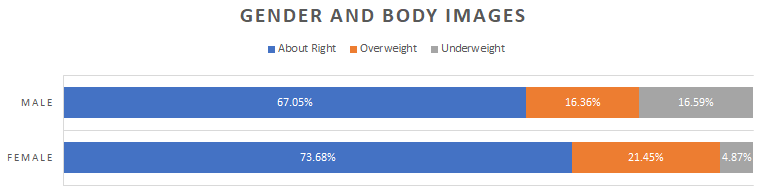
\includegraphics[width=0.9\linewidth]{Figures/Gender-Body.png}
  }}
\end{fullwidth}

\end{example}
\vspace*{\baselineskip}

\hypertarget{percentage-reduction-of-risk}{%
\subsection{Percentage Reduction of
Risk}\label{percentage-reduction-of-risk}}

\begin{itemize}
\item
  When calculating the probability of a negative outcome, we often refer
  to the probability as a \textbf{risk}.
\item
  In general, we are interested in determining how much a new treatment
  reduces the risk compared to a reference risk
\item
  The \textbf{percentage reduction of risk} is
\begin{fullwidth}
  \begin{flushright}
    \colorbox{white}{
    $\text{percentage reduction of risk}=\dfrac{\text{new treatment risk}-\text{reference risk}}{\text{reference risk}}.$
  } 
  \end{flushright}
\end{fullwidth}
\end{itemize}

\begin{example}

Researchers in the Physicians' Health Study (1989) designed a randomized
double-blind experiment to determine whether aspirin reduces the risk of
heart attack. Here are the final results.

\begin{longtable}[]{@{}
  >{\centering\arraybackslash}p{(\columnwidth - 6\tabcolsep) * \real{0.2209}}
  >{\centering\arraybackslash}p{(\columnwidth - 6\tabcolsep) * \real{0.2791}}
  >{\centering\arraybackslash}p{(\columnwidth - 6\tabcolsep) * \real{0.3140}}
  >{\centering\arraybackslash}p{(\columnwidth - 6\tabcolsep) * \real{0.1860}}@{}}
\toprule()
\begin{minipage}[b]{\linewidth}\centering
\end{minipage} & \begin{minipage}[b]{\linewidth}\centering
\textbf{Heart Attack}
\end{minipage} & \begin{minipage}[b]{\linewidth}\centering
\textbf{No Heart Attack}
\end{minipage} & \begin{minipage}[b]{\linewidth}\centering
\textbf{Row Totals}
\end{minipage} \\
\midrule()
\endhead
\textbf{Aspirin} & 139 & 10,898 & 11,037 \\
\textbf{Placebo} & 239 & 10,795 & 11,034 \\
\textbf{Column Totals} & 378 & 21,693 & 22,071 \\
\bottomrule()
\end{longtable}

\emph{Does aspirin lower the risk of having a heart attack?}

\end{example}
\vspace*{6\baselineskip}

\hypertarget{hypothetical-two-way-tables}{%
\subsection{Hypothetical Two-way
Tables}\label{hypothetical-two-way-tables}}

A \textbf{hypothetical two-way table}, also known as a hypothetical 1000
two-way table, is a two-way table constructed from given probability
conditions with 1000 or higher as the total frequency. It can be used to answer
complex probability questions.

\begin{example}

A pregnant woman often opts to have an ultrasound to predict the gender
of her baby. Assume the following facts are known:

\begin{itemize}
\item
  Fact 1: 48\% of the babies born are female.
\item
  Fact 2: 90\% of girls were correctly identified.
\item
  Fact 3: 75\% of boys were correctly identified.
\end{itemize}

Use the above facts to answer the following questions.

\begin{enumerate}
\item
  If the examination predicts a girl, how likely the baby will be a
  girl?
\item
  If the examination predicts a boy, how likely the baby will be a boy?
\end{enumerate}

\end{example}

\begin{exercise}

The table below is based on a 1988 study of accident records conducted
by the Florida State Department of Highway Safety. 

\begin{tabular}{*{4}{l}}
  \hline
  &\textbf{Nonfatal}~ &\textbf{Fatal}~
    &\textbf{Row Totals}~  \\
    \hline
    \textbf{Seat Belt}
  & 412,368 & 510 & 412,878\\
  \textbf{No Seat Belt} & 162,527 & 1,601
  & 164,128\\
  \textbf{Column Totals}
  & 574,895 & 2,111 & 577,006\\
  \hline
\end{tabular}

\emph{Does wearing a seat belt lower the risk of an accident resulting
in a fatality?}

\end{exercise}
\vspace*{6\baselineskip}

\begin{exercise}

A large company has instituted a mandatory employee drug screening
program. Assume that the drug test used is known to be 99\% accurate.
That is, if an employee is a drug user, the test will come back positive
(``drug detected'') 99\% of the time. If an employee is a non-drug user,
then the test will come back negative (``no drug detected'') 99\% of the
time. Assume that 2\% of the employees of the company are drug users.

If an employee's drug test comes back positive, what is the probability
that the test is wrong and the employee is in fact a non drug user?

\end{exercise}
\vspace*{6\baselineskip}

\hypertarget{create-stacked-bar-chart-in-excel}{%
\subsection{Create Stacked Bar Chart in
Excel}\label{create-stacked-bar-chart-in-excel}}

To create a a stacked bar chart of a two-way table

\begin{itemize}
\item
  First select the data table.
\item
  Look for and click \texttt{Insert\ Column\ or\ Bar\ Chart} in the
  menu \texttt{Insert} $\rightarrow$ \texttt{Charts}.
\item
  In the dropdown menu, choose the third option in 2-D Column
  (\texttt{100\%\ Stacked\ Column}) or the third option 2-D Bar
  (\texttt{100\%\ Stacked\ Bar}).
\item
  To switch row/column, in the output graph, right click the row axis
  or the column axis, and chose the option \texttt{Select\ Data...} to
  make a switch.
\end{itemize}
\begin{exercise}

The following table summarize results from a study on program selection
and gender.\\
\begin{fullwidth}
  \colorbox{white}{
    \parbox{\linewidth}{\centering
  \begin{tabular*}{0.9\linewidth}{l*{7}{p{0.08\linewidth}}}
  \toprule
  & Arts-Sci
  & Bus-Econ
  & Info Tech
  & Health Science
  & Graphics Design
  & Culinary Arts
  & Row Totals
  \\
  \midrule
  Female & 4,660 & 435 & 494 & 421 & 105 & 83 & 6,198 \\
  Male & 4,334 & 490 & 564 & 223 & 97 & 94 & 5,802 \\
  Column Totals & 8,994 & 925 & 1,058 & 644 & 202 & 177 & 12,000 \\
  \bottomrule
  \end{tabular*}
  }}
\end{fullwidth}

Use Excel to answer the following question about the study.

\begin{enumerate}
\item
  Is there an association between gender and program selection? Why or
  why not?
\item
  If they are associated, is the association strong or week?
\end{enumerate}

\end{exercise}

